\chapter{Performance of methods for action selection}
When an agent faces several actions whose rewards are unknown, it must balance two goals: try actions that look good right now (exploit) and try other actions to learn if they might be even better (explore). Different strategies — from pure randomness to careful optimism — handle that tradeoff in different ways. Comparing these strategies systematically is how we decide which are useful in practice.

There are four families of simple strategies we use as baselines or building blocks.
\begin{itemize}
    \item \textit{Random action selection.} This is the simplest: pick any action with equal probability.
    \item \textit{Greedy.} Always pick the action with the highest current estimated value.
    \item \textit{$\epsilon$-greedy.} Mostly act greedily, but with small probability $\epsilon$ pick a random action.
    \item \textit{Optimistic initial values.} Initialize the estimated values of all actions to a high number so that, even if you act greedily according to those estimates, every action will be tried at least a few times (because the optimistic estimates will be reduced once you observe reality).
\end{itemize}

\section{The 10-armed testbed}
To compare action-selection methods fairly and repeatably we use a canonical simulated environment called the 10-armed bandit testbed. It’s small (10 actions) but random enough to be a useful benchmark.

For each independent bandit problem, each action $a$ is assigned a true value $q_*(a)$. Those true values are drawn independently from a normal distribution with mean 0 and variance 1.
When the agent selects action $a$, the observed reward is a noisy sample centered on $q_*(a)$. Specifically, the actual reward $R$ is drawn from a normal distribution with mean $q_*(a)$ and variance 1.
So each run is a realization of a random problem: first the vector $q_*(1\ldots 10)$ is drawn; then, as the agent acts, individual rewards are drawn around the selected action’s mean (see Figure \ref{fig:10-arms-testbed}).

\begin{figure}[ht]
    \centering
    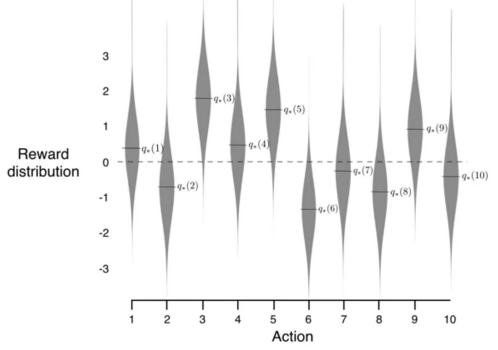
\includegraphics[width=0.7\linewidth]{images/10-arms-testbed.png}
    \caption{10-arms testbed.}
    \label{fig:10-arms-testbed}
\end{figure}

There are three separate sources of randomness that matter:
\begin{itemize}
    \item The true action values $q_*$ are random from one run to the next. Every independent run uses a different underlying bandit problem.
    \item Given $q_*$, the rewards the agent observes are random because of the Gaussian reward noise.
    \item If the action-selection policy performs exploration (e.g., $\epsilon$-greedy or random selection), those exploration steps are themselves random.
\end{itemize}
To obtain a stable picture of performance we perform many independent runs. The classic setup used here is 2000 independent runs of a 10-armed bandit, each run lasting 1000 time steps. For each time step $t$ we average the reward received, using the the sample-average method, across the 2000 runs. This averaged curve smooths out per-run noise and reveals the learner’s average behavior over problems (see Figure \ref{fig:avg-run}).

When we average over 2000 runs, two phases usually appear in the reward-per-step curve. First, an early learning period where reward increases sharply as the agent discovers better actions. After that, the curve levels off toward a steady value that represents the long-run average reward for that algorithm in this testbed.

Across experiments, a consistent pattern emerges: the purely greedy algorithm ($\epsilon$ = 0) tends to perform poorly in the long run because it can get stuck on suboptimal actions discovered early. By contrast, small amounts of exploration ($\epsilon$ = 0.01 or $\epsilon$ = 0.1) allow continual sampling of other actions and better long-term performance (see Figure \ref{fig:agv-egreedy}).
On the particular testbed used in these experiments, the greedy method achieved an average reward per step of about 1.0, whereas the best possible average reward for that testbed is around 1.55. Adding exploration with $\epsilon$ = 0.1 moves the agent closer to that optimum.

\begin{figure}[ht]
    \centering
    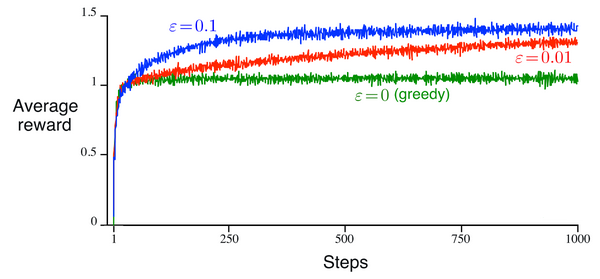
\includegraphics[width=0.7\linewidth]{images/agv-egreedy.png}
    \caption{Performance comparison between greedy and $\epsilon$-greedy.}
    \label{fig:agv-egreedy}
\end{figure}

Let's compare greedy ($\epsilon$ = 0 with optimistic initialization $Q_1(a)=+5$ and $\epsilon$ = 0.1 (regular $\epsilon$-greedy) to see how optimistic initialization changes behavior (see Figure \ref{fig:avg-optimistic}).

$\epsilon$ = 0.1 usually performs much better long run because it keeps exploring 10\% of the time. Optimistic initial values with greedy action selection can approximate the exploration of an $\epsilon$-greedy agent during the initial time steps: agents try many actions early because of the initial optimism. However, after that initial exploration period the agent behaves greedily and will not continue to explore, so long-term performance depends on whether that initial exploration found the best action.

\begin{figure}[ht]
    \centering
    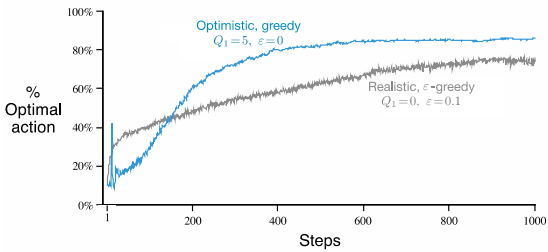
\includegraphics[width=0.7\linewidth]{images/avg-optimistic.png}
    \caption{Performance comparison between $\epsilon$-greedy and optimistic initial value.}
    \label{fig:avg-optimistic}
\end{figure}

\section{Optimism in the Face of Uncertainty}
There are several simple ways to push an agent away from pure greed and make it explore.
A more subtle and powerful principle is \textit{“optimism in the face of uncertainty.”} The idea is not merely to prefer actions whose current estimated means are high, nor to prefer actions you haven’t tried at all. Instead, prefer actions that have the greatest potential to be the best, i.e., those that have high upper bounds on their plausible true value because we’re still uncertain about them.

Think about two simple toy problems. First, a very easy one: two arms, one always good and one always bad. Try both once and you’re done; you’re certain which is best. Now a harder one: two arms where one is slightly better than the other, but rewards are noisy. Here it may take a very long sequence of samples to confidently tell which mean is higher. Hard problems are those where arms have similar true means and the observation noise is large.

We can picture uncertainty as a confidence interval around our current estimate $Q(a)$ (see Figure \ref{fig:confidence-interval}). If that interval is tiny, we’re pretty sure $q_*(a)$, the true mean, is near $Q(a)$. If it’s large, all we know is that the true mean might still be much higher (or lower) than our estimate. The width of that interval shrinks with more samples.

\begin{figure}[ht]
    \centering
    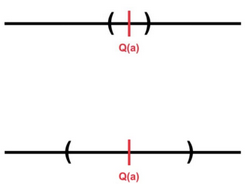
\includegraphics[width=0.4\linewidth]{images/confidence-interval.png}
    \caption{Confidence interval.}
    \label{fig:confidence-interval}
\end{figure}

If an action’s estimated mean is modest but its uncertainty interval stretches well above the other actions’ current values, that action has the potential to be the best. Optimism in the face of uncertainty says: treat that potential as real until we’ve shown otherwise. In practice this leads us to pick actions not simply by their point estimates but by optimistic upper estimates — the highest plausible value consistent with the data so far.

Imagine you’re looking at three arms (see Figure \ref{fig:ucb-graph}). One has a high estimated mean but a tight confidence interval (green line); the second has a slightly lower estimate but a wide interval (blue line); the third is poorly sampled and its interval reaches the highest possible values (red line). Choosing the arm with the highest upper bound either gives you a good reward immediately if the optimism was justified, or it teaches you the most about uncertain arms if the optimism turns out to be wrong. Both outcomes are valuable.

\begin{figure}[ht]
    \centering
    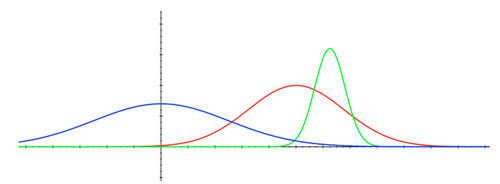
\includegraphics[width=0.7\linewidth]{images/ucb-graph.png}
    \caption{Optimism in the face of uncertainty plot example.}
    \label{fig:ucb-graph}
\end{figure}


Upper Confidence Bound action selection makes the optimism concrete. At time step $t$ pick the action $a$ that maximizes
\begin{equation*}
    A_t = argmax_a\left[Q_t(a) + c\sqrt{\frac{\ln{t}}{N_t(a)}}\right]
\end{equation*}
where: $Q_t(a)$ is your current estimate (sample average, for instance) of action $a$'s mean reward at time $t$. $N_t(a)$ is the number of times action $a$ has been selected so far (at time $t$). $\ln{t}$ is the natural logarithm of the current global time step; it grows slowly with time.
$c$ is a positive parameter you choose that scales how optimistic you are — larger $c$ means more exploration. The second term is the “exploration bonus” or “upper-confidence term.” It decreases as $N_t(a)$ grows, roughly like $1/N_t(a)$, so the more you try an action, the less extra credit you give it for uncertainty. The log factor $\ln{t}$ makes the bonus shrink slowly with overall time so that arms that were neglected a long time ago get a slowly increasing chance relative to others (but not too rapidly).

\begin{Example}{Exploration term}{}
Suppose we are at global time step $t=10,000$. For an action $a$ that has been chosen $N_t(a)=5,000$, the uncertainty term becomes $\sqrt{\frac{\ln{10000}}{5000}}\approx 0.043$. If another action has been chosen only 100 times, the term is $\sqrt{\frac{\ln{10000}}{100}}\approx 0.303$. 

That shows how the UCB bonus strongly favors less-sampled actions and how the magnitude depends on the counts. So if $c=1$, the less-sampled action would have a bonus of about 0.3 while the well-sampled action gets 0.043. With a larger $c$ you amplify the preference for uncertainty.
\end{Example}

$\epsilon$-greedy will forever pick a random action at rate $\epsilon$ (for example 10\% of the time if $\epsilon$ = 0.1), while UCB tends to front-load exploration: it explores a lot initially to reduce uncertainty about all arms and then gradually reduces exploration as confidence grows. UCB’s exploration decreases with time because the upper-confidence bonuses shrink as sample counts increase. This leads to strong performance on stationary problems where the action means don’t change.



\begin{figure}[ht]
    \centering
    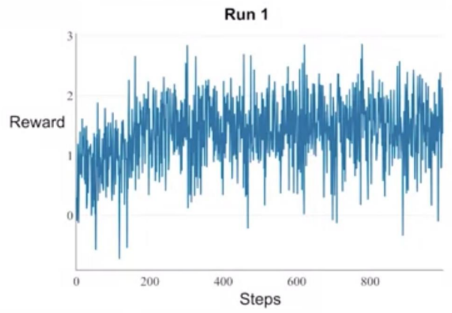
\includegraphics[width=0.6\linewidth]{images/avg-run1.png}
    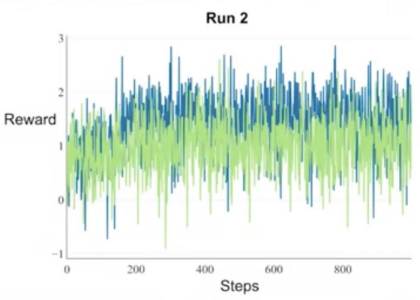
\includegraphics[width=0.49\linewidth]{images/avg-run2.png}
    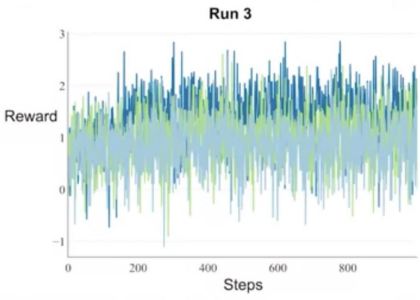
\includegraphics[width=0.49\linewidth]{images/avg-run3.png}
    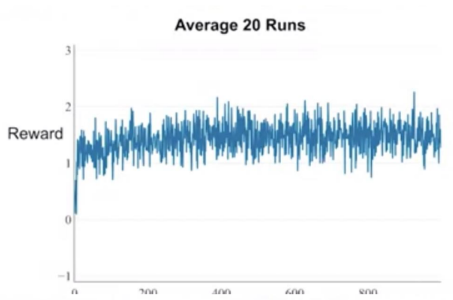
\includegraphics[width=0.49\linewidth]{images/avg-run20.png}
    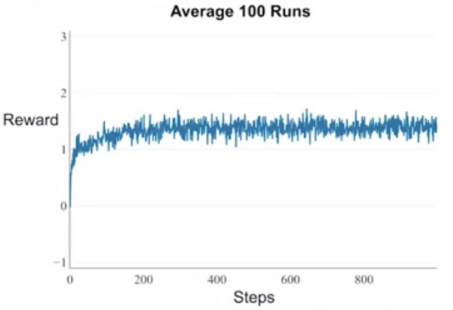
\includegraphics[width=0.49\linewidth]{images/avg-run100.png}
    \caption{Multiple runs in the 10-arms testbed.}
    \label{fig:avg-run}
\end{figure}